% This is samplepaper.tex, a sample chapter demonstrating the
% LLNCS macro package for Springer Computer Science proceedings;
% Version 2.20 of 2018/03/10
%
\documentclass[conference]{IEEEtran}
\IEEEoverridecommandlockouts

\usepackage[T1]{fontenc}
\usepackage{amsfonts}
\usepackage{xcolor}
\usepackage{acronym}
\usepackage{amsmath}
\usepackage[ruled]{algorithm2e}
\def\doi#1{\href{https://doi.org/\detokenize{#1}}{\url{https://doi.org/\detokenize{#1}}}}
%
\usepackage{graphicx}

% Used for displaying a sample figure. If possible, figure files should
% be included in EPS format.
%
% If you use the hyperref package, please uncomment the following line
% to display URLs in blue roman font according to Springer's eBook style:
% \renewcommand\UrlFont{\color{blue}\rmfamily}
%
\usepackage{listings}

\usepackage{cleveref}
\lstset{language=Pascal}
\begin{document}
%
\title{Field-informed Reinforcement Learning for Learning Large-Scale Collective Tasks} %% Todo improve
% or: Field-Informed Reinforcement Learning: A Scalable and Effective Method for Collective Intelligence
% or: A Novel Approach to Reinforcement Learning for Adaptive Collective Systems
%

\author{
\IEEEauthorblockN{Gianluca Aguzzi}
\IEEEauthorblockA{
%\textit{Department of Computer Science and Engineering} \\
\textit{%Alma Mater Studiorum--
Alma Mater Studiorum — Università di Bologna}\\
Cesena, Italy\\
gianluca.aguzzi@unibo.it
}

\and
%\linebreakand %\and
\IEEEauthorblockN{Mirko Viroli}
\IEEEauthorblockA{
%\textit{Department of Computer Science and Engineering} \\
\textit{%Alma Mater Studiorum--
Alma Mater Studiorum — Università di Bologna}\\
Cesena, Italy\\
mirko.viroli@unibo.it % 0000−0003−2702−5702
}
\and
\IEEEauthorblockN{Lukas Esterle}
\IEEEauthorblockA{
%\textit{Department of Computer Science and Engineering} \\
\textit{%Alma Mater Studiorum--
Aarhus University}\\
Aarhus, Denmark\\
lukas.esterle@ece.au.dk}
}
%
\maketitle              % typeset the header of the contribution
%

\lstdefinelanguage{scala}{
  keywords={abstract,case,catch,class,def,%
    do,else,extends,false,final,finally,%
    for,if,implicit,import,match,mixin,%
    new,null,object,override,package,%
    private,protected,requires,return,sealed,%
    super,this,throw,trait,true,try,lazy,%
    type,val,var,while,with,yield,forSome},
  otherkeywords={=>,<-,<\%,<:,>:,\#},
  sensitive=true,
  morecomment=[l]{//},
  morecomment=[n]{/*}{*/},
  morestring=[b]",
  morestring=[b]',
  morestring=[b]""",
  basicstyle=\lst@ifdisplaystyle\small\fi\ttfamily,
  emphstyle=\bfseries
}
\definecolor{ddarkgreen}{rgb}{0,0.5,0}
\lstdefinelanguage{scafi}{frame=single,basewidth=0.5em,language={scala},
keywordstyle=\color{blue}\textbf, commentstyle=\color{ddarkgreen},
keywordstyle=[2]\color{red}\textbf, keywords=[2]{rep,nbr,foldhood,foldhoodPlus,aggregate,branch,spawn,mux,mid},
keywordstyle=[3]\color{gray}, keywords=[3]{Me,AroundMe,Everywhere,Forever}, %,@@,@@@
keywordstyle=[4]\color{red}\textbf, keywords=[4]{in,out,rd},
keywordstyle=[5]\color{violet}, keywords=[5]{evolve,when,andNext,workflow,G,C,broadcast,gradient,gossip},
keywordstyle=[6]\color{orange}, keywords=[6]{Available,Serving,Done,Waiting,Removing,None,Set}}


\lstset{language={scafi}}
%%% Comment command, to be removed before submission
\newcommand{\meta}[3]{\textcolor{#1}{\textbf{#2}: #3}}
\newcommand{\ga}[1]{\meta{red}{GA}{#1}}
\newcommand{\lukas}[1]{\meta{purple}{Lukas}{#1}}
\newcommand{\mv}[1]{\meta{green}{MV}{#1}}
%% ACRONYMS
\acrodef{DecPOMDP}[DecPOMDP]{decentralized partially observable Markov decision processes}
\acrodef{RL}[RL]{reinforcement learning}
\acrodef{MARL}[MARL]{multi-agent reinforcement learning}
\acrodef{MAARL}[ManyRL]{many-agent reinforcement learning}
\acrodef{MDP}[MDP]{Markov Decision Process}
\acrodef{MLP}[MLP]{multi-layer perceptron}
\acrodef{GNN}[GNN]{graph neural network}
\acrodef{CNN}[CNN]{convolutional neural network}
\acrodef{CTDE}[CTDE]{centralized training and decentralized execution}
\acrodef{DQN}[DQN]{Deep Q-Learning}
\ga{Page limit: 10 pages (include refs)}

\begin{abstract}
%Coordinating a group of autonomous intelligent agents in multi-agent systems to achieve a common, global goal requires them to acquire information locally, share their knowledge, and act accordingly on their environment. 
%
%From this shared knowledge distributed intelligence emerges, enabling the collective of agents to operate together.
%With the rising number of such autonomous agents within these systems, 
% sharing knowledge becomes a dedicated challenge. 
% Here, the individual agents need to control how they share their knowledge in order to not overburden the network or other agents with unnecessary information.
% is a research problem that has been addressed for a long time, 
% due to the challenges posed by distribution and the definition of distributed intelligence. 
%
%The problem is even more evident in collective adaptive systems, 
% where the scale of the systems considered makes the definition of collective behaviours even more challenging. 
%
Coordinating a multi-agent system of intelligent situated agents is a traditional research problem, 
impacted by the challenges posed by the very notion of distributed intelligence.
These problems arise from agents acquiring information locally, sharing their knowledge, and acting accordingly in their environment in order to achieve a common, global goal.
%
Individual agents need to control how they share their knowledge in order to not overburden the network or other agents with unnecessary information.
These problems are even more evident in large-scale collective adaptive systems, where agent interactions are necessarily proximity-based, thus making the emergence of controlled global collective behaviour harder.

In this context, two main approaches have been proposed for creating distributed controllers out of macro-level task/goal descriptions: 
 \emph{manual design}, in which programmers build the controllers directly, and 
 \emph{automatic design}, which involves synthesizing programs using machine learning methods.
%
In this paper, we consider a new \emph{hybrid} approach called  \emph{Field-Informed reinforcement learning}. We utilise manually designed \emph{computational fields} (globally distributed data structures) to manage the interaction between agents. Using \emph{Deep Q-learning} in combination with \emph{Graph Neural Networks} we enable the agents to learn the necessary local behaviour automatically to solve collective tasks. 
%
This allows us to create distributed controllers informed by a collective knowledge 
 that has been distilled during learning, but that uses only local information at runtime.
% 
We demonstrate the effectiveness of this new approach in simulated use cases 
 where tracking and covering tasks for swarm robotics are successfully solved. 
\end{abstract}

\begin{IEEEkeywords}
aggregate computing, Graph Neural Networks, and Cyber-Physical Swarms.
\end{IEEEkeywords}
%
%\ga{Paper levels:
%\begin{itemize}
%  \item Distributed collective intelligence
%  \item GNN and field coordination
%  \item Spatial tracking
%\end{itemize}
%}
\section{Introduction}

Autonomous agents interacting and operating towards a common task, rely on shared information and consequently emerging knowledge in order to achieve the underlying goals efficiently. Coordinating and organising this information exchange within the network of agents is required for improve the collaboration among them further~\cite{jennings1996coordination}. Through this coordination, agents may overcome problems requiring (i) efficiency and accuracy only achieved by multiple agents, (ii) the complimentary competences of the individual agents, or (iii) the collective resources of multiple agents.  

Various phenomena in the real world are not evenly distributed across the environment such as watershed, wild fires, traffic, human crowd movement, or wild life movement from insects, fish, birds, and mammals.
To acquire appropriate information about such phenomena, we also need to distribute the sensors accordingly to cover all aspects sufficiently. While manual deployment will mitigate the problem, not all phenomena are known exactly \emph{a priori} and would require maintenance and adjustment during runtime. Even worse, with phenomena able to change their location, size, and distribution---as it is the case with crowds, wild life, or wild fires---an adaptation of the collective sensors is required in order to keep the required information. 

This leads to several questions 
\begin{enumerate}
	\item How to distribute sensors to ensure good attainment of information?
	\item How to maintain knowledge about the phenomena and unlearn irrelevant information?
	\item How to move sensors when the phenomena moves to ensure good coverage?
\end{enumerate} \lukas{refine and rework these questions}

In this paper, we propose a novel approach combining aggregate computing~\cite{Beal2015Computer} with Graph Neural Networks~\cite{Zhou2020AIOpen} to focus on the relevant areas. We further combine this with reinforcement learning techniques to respond to changing conditions in the environment. 
%
This follows a novel trend in which high-level declarative programming languages are mixed with machine learning techniques in order to synthesise robust collective controllers~\cite{DBLP:conf/acsos/Aguzzi21,DBLP:conf/icdcs/AguzziCV22,DBLP:conf/coordination/AguzziCV22}.
Specifically, 
 our approach utilises aggregate computing to disseminate information by manipulating a computational field, 
 which is a distributed data structure that maps devices to information. 
 This field functions as a dynamic environment in which information is continuously updated and diffused throughout the system. 
 By leveraging this layer, we can build collective distributed intelligence using \ac{GNN},
  which uses the information in the field to determine the best action for a given task.
\ga{first draft, need a refinement}
The remainder of this paper is structured as follows. First, we introduce the relevant background and problem formulation in \Cref{sec:background}. Afterwards, we introduce our approach in \Cref{sec:approach}. \Cref{sec:eval} outlines the performed experiments and discusses the obtained results. Finally, we will present our conclusions in \Cref{sec:conclusion}.


\section{Background and Motivation}
\label{sec:background}
In this section, we aim to provide a concise overview of the system we intend to address, 
 starting with a high-level system model. 
%
We then proceed to discuss relevant research areas that inform our approach. 
%
Finally, we present a formalization of the problem and a discussion of the motivations behind our proposed work.
\ga{Page budget: 1/2 page \\}
%\ga{Plan: discussion about the problem of coordination in multi-agent systems and the need for a scalable approach. In doing this, we will discuss some of the existing approaches (declarative, RL and )}
\subsection{Swarm systems}
This article studies intelligent \emph{collective behaviours} within the context of \emph{large-scale} distributed systems.
 Specifically, we focus on \emph{Cyber-Physical Swarms} or \emph{swarm-like systems}, i.e.,  systems consisting of \emph{devices} (or nodes) equipped with \emph{sensors} and \emph{actuator} able to interact with the real world.
 Each of these nodes can interact with its direct neighbours, either based on physical (e.g. communication range) or logical distance (e.g. 1-hop neighbourhood).
 
%
Each node is governed by an autonomous software agent, executing a \emph{local} control loop. In each iteration of this loop, the agent can access the information available within its own \emph{context}. This context is comprised by information acquired by the node directly through its sensors and the information received from its neighbours. 
%
At the end of each control loop iteration, the node can send messages to its neighbourhood. This message may contain raw sensor data or aggregated information over time or from other neighbours.
% about its current evaluation and update its internal state.
%
%This general model can be adapted to several different scenarios, such as a network of sensors, a network of robots (e.g., swarm robotics), or a network of mobile phones.
Examples of such large-scale system can be a network of robots (e.g., swarm robotics), camera and IoT networks, or a network of mobile phones.
%
Our goal is to find a \emph{homogeneously} distributed controller $\pi$ (i.e., the same controller for the whole system) that, 
 starting from \emph{only} local configurations, leads 
 the system to achieve a certain \emph{collective} requirements through \emph{cooperation}, 
 such as spatial area coverage, phenomena tracking, and node aggregation.
%
The homogeneity of the controller is a key requirement to ensure the \emph{scalability} of the approach, 
 as it allows us to avoid the need for a centralised controller that would be a bottleneck for the system,
 and it is the typical choice in swarm-like systems~\cite{brambilla2013swarm,yang2021many,pmlr-v80-yang18d,DBLP:conf/aaai/ZhengYCZZWY18}.
%
\subsection{Field-based Coordination}
%\ga{discussion about field used as a coordination mechanism in multi-agent systems. Introduction to AC}
The field-based coordination approaches utilise a concept of \emph{computational fields} 
 (or simply \emph{fields}), 
 which are \emph{distributed} data structures that associate locations with values and evolve over time. 
%
\emph{Aggregate computing}~\cite{Beal2015Computer}, a modern field-coordination approach, is rooted in earlier work on \emph{artificial potential fields}~\cite{DBLP:conf/icra/Warren89} and \emph{co-fields}~\cite{DBLP:journals/pervasive/MameiZL04}. 
% 
This \emph{macro-programming}~\cite{DBLP:journals/corr/abs-2201-03473} paradigm can be realised to devise collective and self-organizing behaviour through a composition of functions operating on fields. 
%
The fields map a set of individual agents to computational values, 
 allowing them to associate what they sense, process, and actuate. 
%
Fields are computed locally but subject to a global viewpoint, 
 enabling emergent collective behaviour through the interplay of the \emph{system model} (i.e., structure and dynamics of the systems)
 and the \emph{programming model} (i.e., how collective behaviours are expressed) known as field calculus~\cite{DBLP:conf/esocc/ViroliDB13,DBLP:journals/corr/ViroliADPB16,DBLP:journals/tocl/AudritoVDPB19}.
%
The foster is structurally similar to \emph{swarm-like systems}, 
 as it is composed of a set of \emph{agents} 
 that interact with each other through a \emph{network} of \emph{neighbourhood relations}.
%
The dynamics of each agent follow a local control loop called \emph{round}
 that comprises the following steps:
\begin{enumerate}
  \item \emph{Sense}: the agent acquires information from the environment and collects the messages of its neighbourhood, building a \emph{context};
  \item \emph{Compute}: the agent executes a \emph{program} that computes an \emph{export}, that is a set of values to be sent to the neighbourhood;
  \item \emph{Act}: the agent sends the export to its neighbourhood and updates its internal state acting on the environment.
\end{enumerate}
The proactive and iterative execution of the round by each agent leads to the emergence of collective behaviour specified by the program.

The programming model is ruled by the \emph{field calculus}~\cite{DBLP:conf/esocc/ViroliDB13,DBLP:journals/corr/ViroliADPB16,DBLP:journals/tocl/AudritoVDPB19}, 
 a core language that allows the expression of collective behaviours through the composition of \emph{functions} operating on fields.
%
Field calculus includes main operators for expressing \emph{spatio-temporal} compotations that allow for 
\emph{i)} the progression of values over time, achieved by transforming a value computed in a previous round into a new value; 
\emph{ii)} the exchange of data with neighbouring fields, where received data is validated by adjacent fields; and 
\emph{iii)} the conditional division of computation into distinct domains of collective computation. 
%
We avoid presenting here the full details of these operators since they are not essential to the contribution. 
For further elaboration on the actual field calculus, please refer to the work of~\cite{DBLP:journals/jlap/ViroliBDACP19}.

On these minimal operators, 
 it is then possible to build \emph{self-organizing} coordination blocks.
 One of the founding blocks is the \emph{gradient} essential for 
 \emph{information} flows~\cite{DBLP:conf/saso/WolfH07}.
%
This operator generates a numerical field that represents the minimum distance from a source zone. 
%
In other words, it maps a Boolean field (where ``true'' indicates the presence of a source node and ``false'' indicates its absence) to a distance field that indicates the proximity to the nearest source. In ScaFi (a scala implementation of aggregate computing) it is simply expressed as:
\begin{lstlisting}
def gradient(source: Boolean): Double
\end{lstlisting}
Along the gradient, it is possible to cast information within the system, accumulating value during the programming. This pattern is called \emph{gradient-cast} (or \emph{G}) 
\begin{lstlisting}
def G[V](source: Boolean, value: V, acc: V => V): V
\end{lstlisting}
\ga{more description here}
this is used in the use case to accumulate the distance from the phenomena that is tracked
\lukas{still not sure how the coordination works or if it has been explained in the above paragraph.}
\subsection{Graph Neural Networks}
%Over the years, several different neural networks have been proposed to solve specific tasks, ranging from 
%  simple \ac{MLP}~\cite{werbos1975beyond} to \ac{CNN}~\cite{oshea2015introduction}.
%  \lukas{more examples? }
%%
%Whereas \ac{CNN} is designed to be used with image and spatial-like data (e.g., audio), 
 \ac{GNN} is a novel neural network model used to process graph-structured data with deep learning approaches.
%
Let $G = (V, E)$ a graph  
where $E$ defines the neighbourhood relations for each participating node, 
and $V$ identifies the nodes present in the graph. %at that time.  \lukas{no time in the definition}
% 
Each node $v \in V$ is associated with an observation (or feature set) $o_v$.
%\lukas{Over time this graph $G$ can change and therefore we define $G_t$ as the graph $G$ at a specific time $t$.} 
%
Given $o_v$, %a feature vector associated with each node $v \in V$, 
 the goal of a \ac{GNN} is to learn the node embedding $h_v$ for each node $v \in V$. The node embedding $h_v$ describes the node in the network and summarises the geometric properties of the graph in this location, allowing for comparison of various nodes in the graph.
 In modern \acp{GNN}, the node embedding $h_v$ is computed by aggregating information from the node's neighbours $N(v)$,
  and then combining it with the node's current embedding $h_v$.
 The graph is further partitioned into layers with the node $v$ at its bottom layer $0$. With each traversal of an edge $e \in E$ from $v$, the number of layers increased
Formally, a \ac{GNN} can be defined by two phases:
\begin{equation}
a_{v}^{(k)}=\operatorname{AGGREGATE}^{(k)}\left(\left\{h_{u}^{(k-1)}: u \in \mathcal{N}(v)\right\}\right)   
\end{equation}

\begin{equation}
h_{v}^{(k)}=\operatorname{COMBINE}^{(k)}\left(h_{v}^{(k-1)}, a_{v}^{(k)}\right)
\end{equation}
where $h_{v}^{k}$ is the embedding of node $v$ within the $k$-th layer ($h_v^0 = o_v$), 
 $\mathcal{N}(v)$ is the set of neighbours of node $v$ computed from $E$.
%
The differential part comes into play in the $\operatorname{COMBINE}$ function, 
 which is usually a differentiable function such as a neural network layer.
%
$\operatorname{AGGREGATE} $ instead is a function that aggregates the information from the neighbours of a node $v$
  and it could be a simple sum, max or sum of products. More complex aggregation functions are available~\cite{pellegrini2020learning}.
%
This formulation allows GNNs to effectively process and extract features from graph-structured data by iteratively aggregating and transforming information from the node's neighbours.
\lukas{do we need definitions of $o_v$, $h_v^*$ over time $t$?}

\acp{GNN} are used in several application areas such as social network analysis, chemistry, and physics.
In this paper, we use GNNs to learn a local behaviour for each agent in a multi-agent system (more details in Section~\ref{sec:approach}).
\subsection{Many-Agent Reinforcement Learning}
%\ga{plan: we could discuss briefly about standard approach (few agents), and mean-field approach (many agents). 
%This will lead to our approach, which is a combination of DQN (or any Deep RL approach) and GNN.}

 \Ac{RL} has gained a lot of interest recently, 
 thanks to its successful application in various scenarios, 
 ranging from video games (such as Alpha Go~\cite{Silver2016Go} and Atari~\cite{Atari2016DQN}) 
 to chatbots (like ChatGPT~\cite{ChatGPT2023}). 
% 
In \ac{RL}, an \emph{agent} (i.e., a smart entity capable of making decisions) 
 performs \emph{actions} in an \emph{environment} (i.e., everything outside the agent) according to a \emph{policy}, 
 to maximise long-term \emph{reward signal} (or minimise a \emph{regret}).

One interesting application of \ac{RL} is when there are multiple learning agents involved. 
 Such scenarios are referred to as multi-agent reinforcement learning (MARL)~\cite{zhang2019marl}. 
%
In particular, in this work, we consider homogenous \ac{MAARL}~\cite{yang2021many}, 
 where the set of agents $N \gg 2$ and each agent is interchangeable and indistinguishable.
%
This research area is relevant in the context of large-scale systems 
 where collective intelligence emerges from local and repeated interaction of simple entities, like in swarm robotics.
%
In such many-agent scenarios, 
 the implementation of fully decentralized learning is often unfeasible due to the large number of learning agents, 
 which renders the system non-stationary and difficult to manage. 
%
Conversely, a centralized controller capable of coordinating 
 the entire system may not be a viable solution due to scalability concerns. 
 To address this challenge, a practical solution is the adoption of \ac{CTDE}.
%
The idea is to learn a policy at simulation time where there is a collective view of the system, 
 and then at runtime use the policy found with global information. 
This approach allows policies that are influenced by global information but only require local information to function at runtime. 
%
The typical approach in such cases is based on actor-critic systems~\cite{DBLP:conf/nips/LoweWTHAM17,wu2022more,song2022ctds,song2022centralized},
  where the \emph{actor} is the distributed policy (with only local information) and the critic is a neural network that takes the overall system state.
%
%In fact, the first works in this direction were discussed precisely swarm robotics, %\lukas{what does this mean `in the last field'?}
% exploring new models (e.g., swarMDP~\cite{DBLP:conf/atal/SosicKZK17}) and learning algorithms capable of extrapolating a policy representing the entire system.  \lukas{This sentence still needs rework.}
%Modern approaches, however, 
% have started to consider the use of 
% Recently, deep learning approaches have been considered 
% to synthesise robust controllers capable of generalizing to new tasks. 
%In this context, mean-field reinforcement learning~\cite{pmlr-v80-yang18d} is certainly noteworthy. 
Mean-field RL~\cite{pmlr-v80-yang18d} is one of such concrete applications of \ac{CTDE} 
 where the interactions among the population of agents are estimated by considering either the effect of a single agent and the average impact of the entire population or the influence of neighbouring agents.
%
Some known approaches using mean-field reinforcement learning include Q-mean, 
 which is an extension of Q-learning to mean-field settings~\cite{yang2018mean}, 
 and actor-critic mean-field~\cite{frikha2023actor}, which combines actor-critic algorithms with mean-field approximations. 
%
These approaches have shown promising results in various domains, such as multi-agent coordination 
 and decentralised control, and are actively being researched and developed for further applications.
\subsection{Problem formalisation}
Given the homogeneity, large system scale, and the \emph{locality} (i,e., each agent can only observe its neighbours), 
 the problem can be modelled through the SwarMDP model~\cite{DBLP:conf/atal/SosicKZK17} -- 
 an extension of the \ac{DecPOMDP}~\cite{Decpomdp2000} model for swarm-like systems.
% 
A SwarMDP is characterised by a \emph{swarming agent} ($\mathbb{A}$) and the dynamics of the environment ($\mathbb{E}$).
Specifically, $\mathbb{A}$ is a tuple ($\mathcal{S}, \mathcal{O}, \mathcal{A}, \mathcal{R}, \pi$) where:
\begin{itemize}
  \item $\mathcal{S, O, A}$ are the set of local states, observations (or features), and actions, respectively;
  \item $\mathcal{R}: \mathcal{S} \rightarrow \mathbb{R}$ is the reward function, which is influenced by the environment;
  \item $\pi: \mathcal{O} \rightarrow \mathcal{A}$ is the policy function, which maps the observations to the actions. It could be deterministic or stochastic.
\end{itemize}
Starting from this definition, the environment $\mathbb{E}$ is defined as a tuple ($\mathcal{P}, \mathbb{A}, \mathcal{T}, \xi$), where:
\begin{itemize}
  \item $\mathcal{P}$ is the total number of agents in the systems (the agent population), which is assumed to be fixed;
  \item $\mathbb{A}$ is the defined agent prototype that rules each agent $v \in P$;
  \item $\mathcal{T}: \mathcal{S}^P \times \mathcal{A}^P \times \mathcal{S}^P \rightarrow \mathbb{R}$ is the transition  global function, which is influenced by the actions of the agents and returns a collective reward -- this is typically not known by the swarming agents;
  \item $\xi: \mathcal{S^P} \rightarrow \mathcal{O^P}$ is the global observation model of the systems.
\end{itemize}
In swarMDP, the neighbourhood is not directly defined, but it is implicitly defined by the observation model $\xi$.
In our specific case, the agents can only interact with 1-hop neighbourhoods and are not directly influenced by other agent observations. We can therefore restrict the observation model as follows:
\begin{equation}
\xi(v): \{s_j, j \in \mathcal{N}^v\} \rightarrow O
\end{equation}
\begin{equation}
\xi = \{\xi(v), v \in \mathcal{P}\}
\end{equation}
where $\mathcal{N}^v$ is the set of neighbours of $v$.

This model can be used then to express the evolution of the system in time.
Specifically, starting from a global state $\mathcal{S}^P_t$, the next state $\mathcal{S}^P_{t+1}$ is defined as:
\begin{equation}
\mathcal{A}^P_t = \pi(\xi(S^P_t))
\end{equation}
\begin{equation}
\mathcal{S}^P_{t+1} = \mathcal{T}(\mathcal{S}^P_t, \mathcal{A}^P_t)
\end{equation}
Given a time $t$, the system can be also represented as a graph $G_t = (V_t, E_t)$, 
  where $E_t$ is built from $\mathcal{N}$.
  Each node is then decorated with the local observation $o_v$. 
  Therefore, this graph can be used for being processed by a \ac{GNN} as done in~\cite{DBLP:conf/corl/TolstayaGPP0R19,tolstaya2020learning,DBLP:conf/icra/GosrichMLPYR022}.
\subsection{Motivation}
The definition of distributed controllers for intelligent systems can be divided into two major approaches: 
 \emph{manual design}, where the application is conceived and described through a programming language, 
 and \emph{automatic design}~\cite{brambilla2013swarm}, which employs machine learning techniques to synthesise distributed controllers. 
%
Our work lies between these two approaches, specifically in the areas of field-based coordination and \ac{MAARL} with the use of \acp{GNN}.

Compared to earlier works on field-based coordination, 
 our approach builds on the concept of co-fields~\cite{DBLP:journals/pervasive/MameiZL04}, 
 where agents exploit the field as a stigmergic medium to receive system-wide information and apply reasoning to this data.
%  
We present a subsequent approach where agent intelligence is synthesised through \ac{MAARL} and the use of \ac{GNN} to learn a local representation from the neighbourhood.
%
By learning a smart policy directly in the environment, the agent becomes capable of adapting its behaviour to new situations.

The use of \acp{GNN} as part of a distributed controller has been explored in previous literature~\cite{DBLP:conf/icra/GosrichMLPYR022,DBLP:conf/corl/TolstayaGPP0R19}, 
 where it was shown that they could be used to break down the evaluation of local and distributed systems. 
%
However, in these works, communication was left entirely to the neural network, 
 making the learning process potentially more complex and unstable. 
 In our approach, the \ac{GNN} is \emph{informed} by computational fields that collect the necessary information to compute a certain task, 
 limiting learning to only the specific task defined by a collective reward function.
 This will speed up the learning process and make it more stable.
\section{Field-informed Reinforcement Learning}
\label{sec:approach}
\ga{Page budget: 2/3 pages \\}
%\ga{Plan: we should discuss the approach in detail, including the system model, and the learning dynamics. Particularly, I would like to highlight how each node in the graph is a local controller, but it could be seen as a global evolution, therefore we can use global information to inform the local controller.}
\begin{figure}
  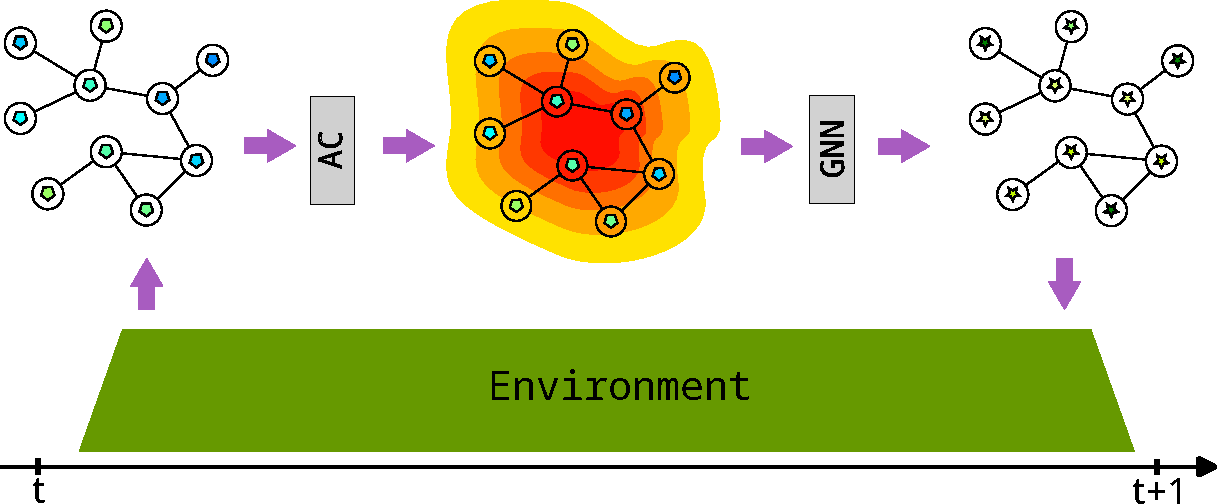
\includegraphics[width=\linewidth]{imgs/architecture.pdf}
  \label{fig:architecture}
  \caption{High-level description of Field-Informed reinforcement learning dynamics. 
  For each time step $t$, a graph is constructed from the environment, and it will associate each node with a local feature (hexagons in the picture). 
  Using this feature, an aggregate program computes spatio-temporal information that enhances the feature set of each node, depicted as colours in the middle graph. 
  Finally, utilizing the GNN, actions are computed for each node in the system to be performed against the environment, enabling advancement in the simulations according to swarMDP rules.
  %\lukas{should we have numbers at each step in the figure (and then referring in the caption and text)?}
  %\lukas{also, i think we can have the AC and GNN box a bit smaller but increase the size of the networks slightly - and put it on column width ot save space}
}
\end{figure}
In this section, we aim to clarify the components involved in our proposed solution (i.e., architecture), how these components interact with each other to bring the system to perform the collective behaviour (i.e dynamics), and finally, we will detail the learning algorithm designed and used to synthesise the policy (learning algorithm).
\subsection{Architecture and System dynamics}
%\ga{Plan: 
%  discussion about the typical AC evaluation model, specifying how GNN (with 1-hop information diffusion)
%  can be easily integrated with this distributed model
%}
The proposed solution consists mainly of two parts, 
\emph{i)} the aggregate program used to create part of the observation and 
\emph{ii)} the policy $\pi_{gnn}$ learned through \ac{GNN}-based approach. 
%
Let $\Gamma$ be the aggregate program that takes $G_t$ as input. 
% \lukas{$G_t$ is not defined. also, not sure what `runs against' means - take $G_t$ as input?}
%\ga{In the problem formalization, I defined $G_t$, but it may be more appropriate to define it directly in the GNN, as suggested. I made this choice since GNNs typically only receive a graph as input, without regard for time, I included the definition of $G_t$ in the problem formalization as it pertains to the dynamics of the overall system. Specifically, when discussing the system's dynamics at a given time t, it's necessary to define the corresponding graph. I hope this clarifies my reasoning. Let me know!}
%
The evaluation of $\Gamma$ produces a field value $\theta^v_t$ for each node $v$ in $G_t$. 
The feature vector $o_v$ of which is composed the graph $G'_t$ used by the policy $\pi_{gnn}$ is described by:
 $o_v = (\theta^v_t, \omega)$.
 where $\omega$ are other local information gather from sensors (like temperature, distances from neighbourhood, etc.). 
%
The policy $\pi_{gnn}$ is then evaluated for each node, 
 producing an action $a_t$ that will then modify the global state of the system.
 \ga{todo: put pseudo code to express this dynamics}
%
Despite appearing centralised, this system proposes a completely decentralised execution. 
%
In fact, the program $\Gamma$ is proactively executed at every node, 
and the \ac{GNN} can be locally evaluated using only neighbourhood information. 
%
We want to emphasise that, in this case, the \acp{GNN} must be 1-hop; 
otherwise, they could not have a local interpretation for each node, according to our system model.
\subsection{Learning algorithm}
%\ga{
%  Plan: discuss the chosen approach, that is Centralised Training and Distributed Execution.
%  Particularly, we use DQN in which the neural network is a GNN. So, the dataset consists in a set of graphs,
%  where each graph is a snapshot of the system. 
%  The target is the Q-value of the action taken in the current state.
%  Explain how this can be then used for distributed controllers.
%}
Since we consider swarm-like systems, which are an example of many-agent systems, 
 the proposed approach follows a \ac{CTDE} learning pattern,
 but differently from mean-field approaches and actor-critic solutions,
 we use a value-based approach combined with a \ac{GNN} as a function approximator.
%In swarm-like systems, 
% the typical approach for learning follows a strategy known as \ac{CTDE}. \ga{perhaps it should be introduced in many RL} 
%The idea is to learn a policy at simulation time where there is a collective view of the system, 
% and then at runtime use the policy found with global information. 
%This approach allows policies that are influenced by global information but only require local information to function at runtime. 
%
%The typical approach in such cases is based on actor-critic systems~\cite{DBLP:conf/nips/LoweWTHAM17,wu2022more,song2022ctds,song2022centralized},
%  where the \emph{actor} is the distributed policy (with only local information) and the critic is a neural network that takes the overall system state.
%
Specifically, we leveraged the property of \ac{GNN}s to have a dual interpretation, i.e., to function globally over the entire graph and locally only over the neighbourhood. 
%
As value-based algorithm we relied on \ac{DQN}~\cite{mnih2015playing} \ga{to introduce in many rl??} with two major modifications (see \Cref{alg:dqn}): 
\begin{enumerate}
  \item experience replay stores experiences in the form of \emph{graphs},
  \item the neural network used to compute the Q function is based on a \ac{GNN} with an \ac{MLP} downstream.
\end{enumerate}
The first point is a natural extension because we work on graphs rather than simple values. 
%
For the second point,
 the use of \acp{GNN} allows us to define policies on a variable neighbourhood  that is essential in such systems as this can vary based on the neighbourhood policy,
 and it is known that \acp{GNN} have a certain ability to generalise to new structures and scale with different nodes. 
% 
Additionally, 
 using the overall graph compared to local experiences makes learning more stable as it reduces the non-stationarity of the environment perceived by each node.
% 
 During learning, it is as if we have a \emph{single} agent collectively choosing which action to take (i.e., resulting action graph). 
%
\begin{algorithm}
  \KwIn{Environment $\mathbb{E}$, graph replay buffer $\mathcal{D}$, target network $\theta^{-}$, current network $\theta$, exploration strategy $\epsilon$}
  \KwOut{Trained DQN model $\theta$}

  Initialise $\mathcal{D}$ with random initial transitions;

  Initialise $\theta$ with random weights;

  Set $\theta^{-} \leftarrow \theta$;

  \While{not done}{
  Observe current graph observations $G_o$;

  With probability $\epsilon$ select a random graph action $G_a$, 
  otherwise select $G_a =$ 
  $\{ v \in V, argmax_{a'v} Q(G_o, \theta)[v, a'v]\ ,  E \in G_o \}$;

  Execute the collective action $G_a$ in the environment $\mathbb{E}$ and observe a graph-level reward $G_r$ and the next state $G_o'$;

  Store transition $(G_o,G_a,G_r, G_o')$ in $\mathcal{D}$;

  Sample a batch of graph transitions $(G^i_o,G^i_a,G^i_r,G^i_o)$ 
   from $\mathcal{D}$ and merge them in $(G_o,G_a,G_r,G_o)$;

  Compute the target Q-value for each node in the graph: 
  $y = G_r + \gamma * \max{a'} Q(s'i,a';\theta^{-})$;
  
  Compute the current expetected value for each node in the graph:
  $y^* = Q(s'i,a';\theta)$;

  Update the current network weights using gradient descent: $\theta \leftarrow \theta - \alpha \nabla{\theta} \frac{1}{|G_o|} (y - y^*)^2$;

  Every $C$ steps, update the target network weights: $\theta^{-} \leftarrow \theta$
  ;
  }
  \caption{Deep Q-Network (DQN) with GNN and Graph Replay Buffer}
  \label{alg:dqn}
  \end{algorithm}
    
\section{Evaluation}
\label{sec:eval}
\ga{Page budget: 2 pages \\}
%\ga{Plan: we should discuss the robot aggregation scenario, specifying the state space, the action space, and the reward function.
%I dunno if it makes sense to discuss the variants (i.e., fixed area, two areas and moving area). We will see.}
To test the effectiveness of the proposed approach, 
 we decided to experiment with a case study related to swarm robotics, 
 specifically the tracking and coverage of a spatio-temporal phenomenon, cf. tracking a wildfire 
 or monitoring the water levels in a canal.

\subsection{Scenario}
The proposed simulation consists 
 of a set of robots placed in a 2D space capable of perceiving the intensity 
 of the phenomenon of interest through an installed sensor $\zeta_v$ with $v \in \mathbb{V}$. 
 (e.g., camera, temperature sensor, etc.). 
%
Additionally, each node has a coverage range $\omega$ 
 that describes the area it can monitor. 
 Each drone can only communicate directly with its own neighbourhood $\mathcal{N}$, 
 which in this case depends on a $\mathbb{O}$ range,
From the neighbourhood, 
 each node can also perceive the direction of the other nodes.
%
Each node moves following a certain action composed of two components ($\alpha$, $\theta$) 
 which respectively describe the angle and intensity of the movement (i.e., the velocity vector).
\subsection{Goal}
 The objective of this scenario is to:
\begin{itemize}
\item Maximise the number of drones within the phenomena
\item Minimise the number of drones without a neighbourhood
\item Maximise the coverage of the system
\end{itemize}
 
As we are modelling a reinforcement learning system, 
 these three components must be encoded in a reward function 
 that provides an estimate of the current action taken by a given robot.
 
 Regarding the first point, the reward function is simple and is defined as:
 
 \begin{equation*}
 R^a_{v} = \begin{cases}
  1 & \text{if } \zeta_v > 0 \\
  0 & \text{otherwise} 
 \end{cases}
 \end{equation*}
 
This will lead the system to prefer a configuration in which every node is present in the system. 
%
The second point is important because if the system breaks into many scattered drones, 
 they are not able to move in the environment due to the reduced observability of the system. 
 In this case, the reward is defined as:
 
 \begin{equation*}
 R^{\mathcal{N}}_{v} = \begin{cases}
  1 & \text{if } \mathcal{N} > 0 \\
  0 & \text{otherwise} 
 \end{cases}
 \end{equation*}
 
 Finally, to maximise the coverage, 
  we decided to calculate the maximum and minimum distance of the neighbourhood and give more value in case these two values are similar. 
%
This means that the average distance will tend towards the one expressed by the viewing range of each node:
% 
\begin{equation*}
R^{C}_{v} = \frac{d_{max} - d_{min}}{\mathbb{O}}
\end{equation*}
The final reward function is defined as:
\begin{equation*}
R_{v} = \frac{R^a_{v} + R^{\mathcal{N}}_{v} + R^{C}_{v}}{3}
\end{equation*}
Specifically, we decided to express the signal as a \emph{regret}
  as it is a more general measure of the quality of the action taken by the agent.
It is simplify evaluated as:
\begin{equation*}
R^e_{v} = 1 - R_v
\end{equation*}
%

%\paragraph*{Variant A}
%\paragraph*{Variant B}
%\paragraph*{Variant C}

\subsection{Discussion and Results}
\section{Conclusion and Future Work}
\ga{Page budget: 0.5}
\label{sec:conclusion}

\bibliographystyle{IEEEtran}
\bibliography{bibliography}

\end{document}
